\documentclass{beamer}

% Español
\usepackage[spanish]{babel}
\usepackage[utf8]{inputenc}
\usepackage[T1]{fontenc}

% Tipo de letra
\usepackage{palatino}

% Plantilla
\usetheme{Antibes}
%\usetheme{Berlin}

\usepackage{listings}
\lstdefinestyle{cpp11}{
  belowcaptionskip=1\baselineskip,
  breaklines=true,
  xleftmargin=\parindent,
  language=C++,
  showstringspaces=false,
  basicstyle=\scriptsize\ttfamily,
  keywordstyle=\bfseries\color{green!40!black},
  commentstyle=\itshape\color{purple!40!black},
  identifierstyle=\color{blue},
  stringstyle=\color{orange},
  columns=flexible,
  %inputenconding=utf8,
  extendedchars=true,
  morekeywords=[1]{_Pragma,constexpr,nullptr,alignof,alignas},
  literate=%
    {¿}{{?`}}1
    {á}{{\'a}}1
    {é}{{\'e}}1
    {í}{{\'i}}1
    {ó}{{\'o}}1
    {ú}{{\'u}}1
    {ñ}{{\~n}}1
}

\newcommand{\cppkey}[1]{%
{\color{green!40!black}\textbf{\texttt{#1}}}%
}

\newcommand{\cppid}[1]{%
{\color{blue}\texttt{#1}}%
}

\setbeamertemplate{footline}{
  \leavevmode%
  \hbox{\begin{beamercolorbox}[wd=\paperwidth,ht=2.5ex,dp=1.125ex,leftskip=.3cm,rightskip=.3cm]{author in head/foot}%
    \usebeamerfont{author in head/foot}J. Daniel Garcia -- ARCOS@UC3M (josedaniel.garcia@uc3m.es)
    \hfill
    \insertframenumber/\inserttotalframenumber
  \end{beamercolorbox}}%
  \vskip0pt%
}

\usepackage{tikz}
\usetikzlibrary{positioning}
\usetikzlibrary{arrows}
\usetikzlibrary{mindmap}

\usepackage{pgfplots}
\pgfplotsset{compat=1.5}

\usepackage{tabularx}

\addtobeamertemplate{headline}{}
{% 
\begin{tikzpicture}[remember picture,overlay]
\node[anchor=north east] at (current page.north east) {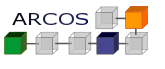
\includegraphics[height=0.7cm]{logos/arcos.png}};
\end{tikzpicture}
}

\addtobeamertemplate{footline}{}
{% 
\begin{tikzpicture}[remember picture,overlay]
\node[anchor=south east,outer ysep=0.8cm] at (current page.south east) {
\includegraphics[height=0.7cm]{logos/techfest.png}};
\end{tikzpicture}
}

  \tikzset{
    invisible/.style={opacity=0},
    visible on/.style={alt=#1{}{invisible}},
    alt/.code args={<#1>#2#3}{%
      \alt<#1>{\pgfkeysalso{#2}}{\pgfkeysalso{#3}} % \pgfkeysalso doesn't change the path
    },
  }

%Portada
\title{Lenguajes nativos versus máquinas virtuales}
\author{J. Daniel Garcia}
\institute{Universidad Carlos III de Madrid}
\date{\today}

\begin{document}

\begin{frame}
\titlepage
\end{frame}

\AtBeginSection[]
{
  \begin{frame}<*>
    \setbeamertemplate{section in toc shaded}[default][50]
    \setbeamertemplate{subsection in toc shaded}[default][50]
    \tableofcontents[currentsection,hideallsubsections]
  \end{frame}
}

\AtBeginSubsection[]
{
  \begin{frame}<beamer>
    \setbeamertemplate{subsection in toc shaded}[default][50]
    \tableofcontents[sectionstyle=show/hide,subsectionstyle=show/shaded/hide]
  \end{frame}
}

\begin{frame}{ADVERTENCIA}
Este material presenta una visión subjetiva.
\vfill
Recoge argumentos recurrentes en conversaciones durante los últimos años con colegas de la industria y la universidad.
\end{frame}

\section{¿Por qué esta charla?}

\begin{frame}[t]{Una conversación real}
  \begin{itemize}
    \item Conversación con empresa líder en su sector.
      \begin{itemize}
        \item ¿Qué tipo de titulados buscas?
        \item Desarrolladores de C/C++.
        \item Últimamente parece que todo el mundo quiere ser desarrollador Java o gestor.
      \end{itemize}
    \item Necesidades:
      \begin{itemize}
        \item Gestión dinámica de memoria.
        \item Gestión de recursos.
        \item Uso extendido de hilos y procesos.
        \item Herramientas de \emph{profiling} y depuración.
        \item Memoria compartida.
        \item Programación paralela.
      \end{itemize}
  \end{itemize}
\end{frame}

\begin{frame}[t]{En busca del lenguaje perfecto}
  \begin{columns}
    \begin{column}{0.3\textwidth}
      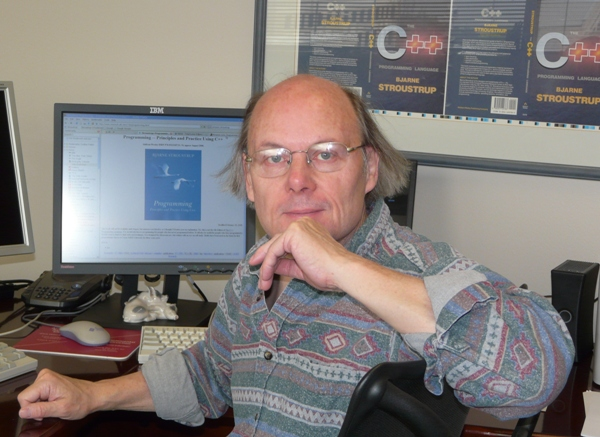
\includegraphics[width=\textwidth]{images/stroustrup.jpg}

      \emph{Bjarne Stroustrup}
    \end{column}
    \begin{column}{0.7\textwidth}
      \begin{quote}
        Anybody who comes to you and says he has a perfect language is either naive or a salesman.
      \end{quote}
      \begin{quote}
        There are only two kinds of languages: the ones people complain about and the ones nobody uses.
      \end{quote}
      \begin{quote}
        People who think they know everything really annoy those of us who know we don't
      \end{quote}
    \end{column}
  \end{columns}
\end{frame}

\begin{frame}[t]{The Perils of Java Schools}
  \begin{itemize}
    \item Don't get me wrong: there's nothing wrong with Java as an implementation language.
      \begin{itemize}
        \item There are lots of things wrong with it but those will have to wait for a different article.
      \end{itemize}
    \item The last decade a large number of otherwise perfectly good schools have gone 100\% Java
    \item {[Programming with pointers]}\ldots is still important for some of the most exciting programming jobs.
    \item Without understanding functional programming, you can't invent MapReduce, the algorithm that makes Google so massively scalable.
  \end{itemize}
  {\tiny
  \url{http://www.joelonsoftware.com/articles/ThePerilsofJavaSchools.html}}
\end{frame}

\section{Lenguajes nativos}

\begin{frame}[t]{Programa nativo}
  \begin{itemize}
    \item Un \textbf{programa nativo} es un programa de computador que se ejecuta directamente en el juego de instrucciones de la máquina.
      \begin{itemize}
        \item Contiene instrucciones de la ISA sobre la que se ejecuta.
        \item No requiere ninguna traducción durante su ejecución.
        \item Puede contener llamadas a un sistema operativo concreto.
      \end{itemize}
  \end{itemize}
\end{frame}

\begin{frame}[t]{Ensamblador}
  \begin{itemize}
    \item Decada de los 40:
      \begin{itemize}
        \item Programas en código máquina codificados directamente comos secuencia de valores binarios.
        \item Aparece la idea de ensamblador.
      \end{itemize}
  \end{itemize}

\begin{columns}
  \begin{column}{0.2\textwidth}
    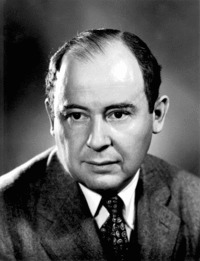
\includegraphics[width=.8\textwidth]{images/von-neumann.jpg}
  \end{column}
  \begin{column}{0.8\textwidth}
    \begin{quote}
      Why would you want more than machine language?
    \end{quote}
    John von Neumann (1903-1957)
  \end{column}
\end{columns}

\begin{itemize}
  \item Aparecen lenguajes ensambladores y herramientas asociadas:
    \begin{itemize}
      \item Ensamblador (assembler): Traduce a código objeto.
      \item Editro de enlaces (linker): Fusiona módulos de código objeto en un ejecutable en código máquina.
    \end{itemize}
\end{itemize}
\end{frame}

\begin{frame}[t]{Problemas con el ensamblador}
\end{frame}

\begin{frame}[t]{Lenguajes de programación}
\end{frame}


\section{La promesa de los lenguajes no nativos}

\begin{frame}[t]{Idea fundamental}
  \begin{itemize}
    \item Write Once Run Everywhere.
      \begin{itemize}
        \item Write Once \textbf{\color{red}Debug} Everywehre.
      \end{itemize}
    \item El compialdor genera un código intermedio independiente del hardware que es leído y ejecutado por una máquina virtual.
    \item Promesa: \textbf{\color{blue}Portabilidad}.
    \item Ejemplos:
      \begin{itemize}
        \item Java.
        \item Familia de lenguajes .NET.
      \end{itemize}
  \end{itemize}
\begin{columns}
  \begin{column}{0.2\textwidth}
    
\includegraphics[width=0.9\textwidth]{images/java.jpg}
  \end{column}
  \begin{column}{0.1\textwidth}
    
\includegraphics[width=0.9\textwidth]{images/dotnet.jpg}
  \end{column}
\end{columns}
\end{frame}

\begin{frame}[t]{Una idea novedosa}
  \begin{itemize}
    \item Idea original en \emph{O-code} de BCPL.
      \begin{itemize}
        \item Finales de los 60.
        \item Permitió portar el lenguaje BCPL a diversas máquinas.
      \end{itemize}
    \item 1966: Lenguaje BCPL.
    \item 1973: \emph{p-code}
      \begin{itemize}
         \item Código de una hipotética máquina virtual.
         \item Generado en la compilación del lenguaje PASCAL.
           \begin{itemize}
             \item Compilación de PASCAL a p-code.
             \item Ejecución del p-code por una máquina virtual.
           \end{itemize}
         \item Posibilidad de construir una implementación hardware de la máquina virtual.
           \begin{itemize}
             \item 1979: PASCAL MicroEngine.
           \end{itemize}
      \end{itemize}
  \end{itemize}
\end{frame}

\begin{frame}[t]{Aspectos de p-code}
  \begin{itemize}
    \item \textbf{\color{blue}Portabilidad}:
      \begin{itemize}
        \item El compilador permanece inalterado.
        \item Solamente se necesita portar el intérprete de p-code.
      \end{itemize}
    \item \textbf{\color{blue}Simplicidad}:
      \begin{itemize}
        \item Se separa la generación de código independiente de la máquina de las características de un procesador concreto.
      \end{itemize}
    \item \textbf{\color{blue}Tamaño}:
      \begin{itemize}
        \item El tamaño del código generado tiene a ser menor que en código máquina nativo.
      \end{itemize}
    \item \textbf{\color{blue}Depuración}:
      \begin{itemize}
        \item El intérprete puede añadir comprobaciones difíciles de implementar en código nativo.
      \end{itemize}
    \item \textbf{\color{blue}Rendimiento}:
      \begin{itemize}
        \item Sobrecarga que puede ser importante.
      \end{itemize}
  \end{itemize}
\end{frame}

\begin{frame}[t]{El caso de Java}
  \begin{itemize}
    \item Desarrollado en 1995 por James Gosling, Mike Sheridan y Patrick Naughton.
    \item Una instancia más de la idea de p-code:
      \begin{itemize}
        \item p-code $\rightarrow$ bytecode.
        \item p-machine $\rightarrow$ Java Virtual Machine.
        \item PASCAL MicroEngine $\rightarrow$ Java Processor (múltiples intentos).
      \end{itemize}
    \item Ideales:
      \begin{enumerate}
        \item Simple, orientado a objetos y familiar.
        \item Robusto y seguro.
        \item Neutral a la arquitectura y portable.
        \item Alto rendimiento.
        \item Interpretado, con hilos y dinámico.
      \end{enumerate}
  \end{itemize}
\end{frame}


\begin{frame}[t]{Un lenguaje robusto}
  \begin{itemize}
    \item Pros:
      \begin{itemize}
        \item Gestión automática de memoria $\Rightarrow$ Para evitar goteos de memoria.
        \item Ocultación de modelo de memoria $\Rightarrow$ Para evitar \emph{dangling references}
        \item Modelo de propagación de excepciones $\Rightarrow$ Para separar la detección y el tratamiento de errores.
      \end{itemize}
    \item Efecto:
      \begin{itemize}
        \item Es difícil que un error haga detenerse un sistema completo.
        \item Pero \ldots
          \begin{itemize}
            \item ¿Quién no ha visto nunca un \texttt{NullPointerException}?
          \end{itemize}
      \end{itemize}
  \end{itemize}
\end{frame}

\begin{frame}[t]{Los goteos de memoria son cosa de C++}
\begin{center}
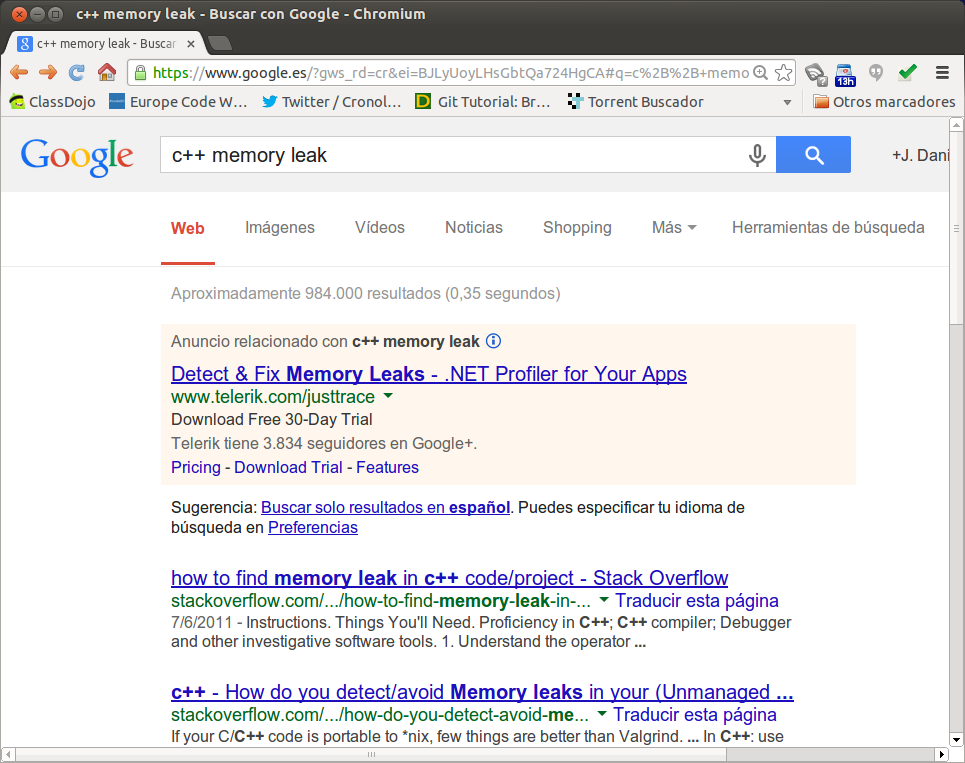
\includegraphics[width=.7\textwidth]{images/cpp-leak.png}
\end{center}
\end{frame}

\begin{frame}[t]{Java resuelve el problema}
\begin{center}
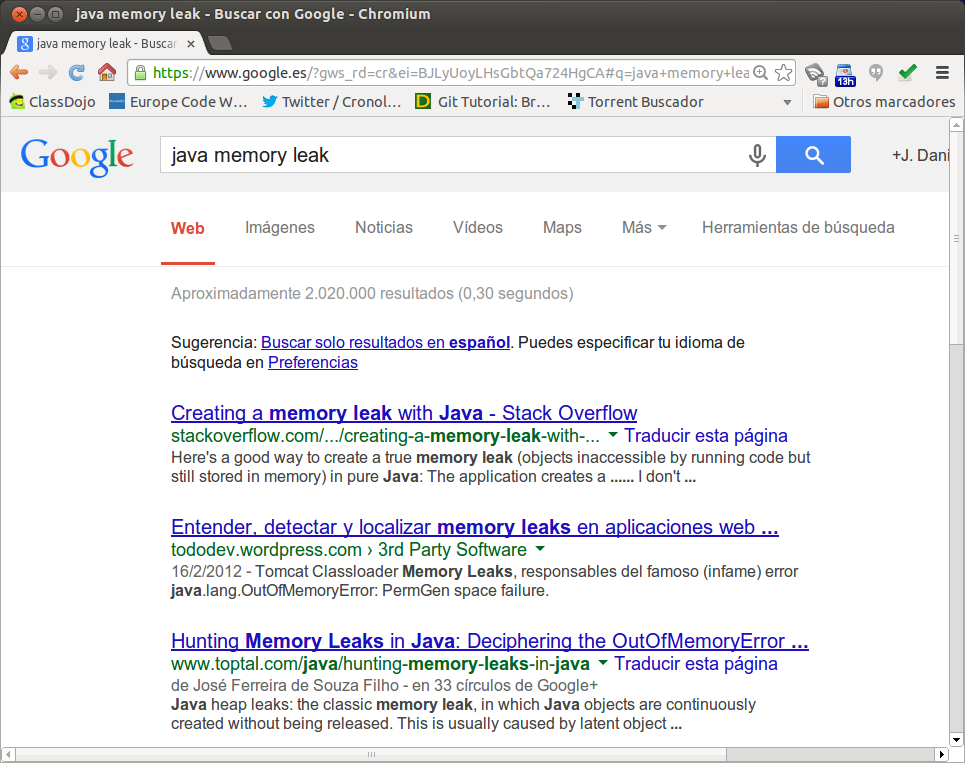
\includegraphics[width=.7\textwidth]{images/java-leak.png}
\end{center}
\end{frame}

\begin{frame}[t]{Pero por lo menos es seguro}
\begin{center}
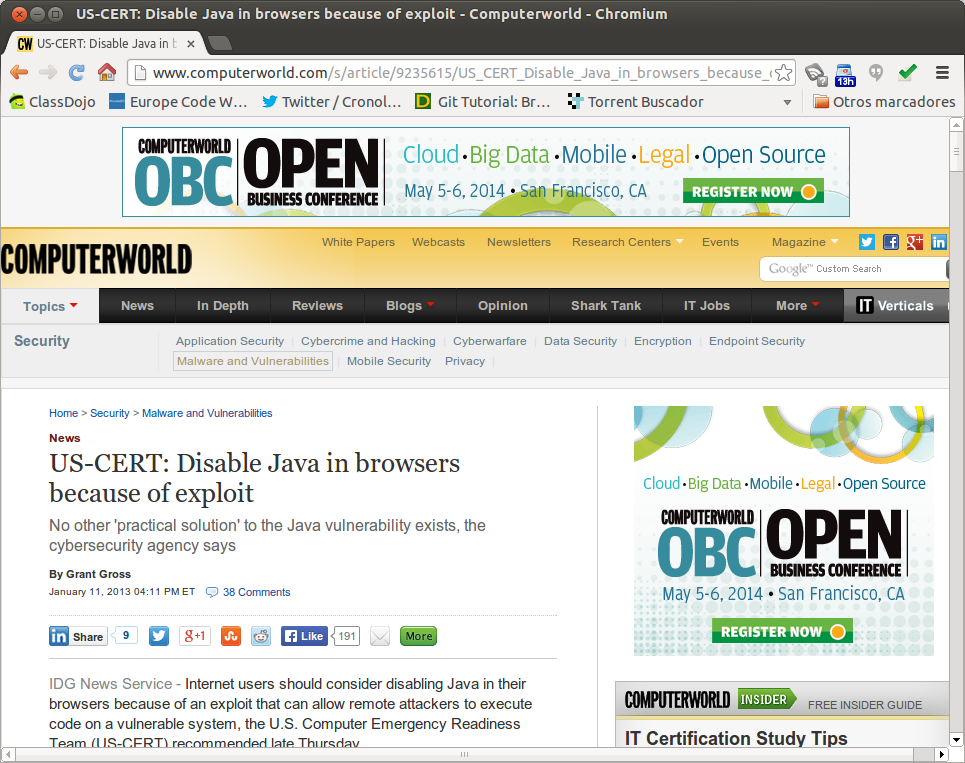
\includegraphics[width=.7\textwidth]{images/java-cert.png}
\end{center}
\end{frame}

\begin{frame}[t]{Alto rendimiento}
\begin{center}
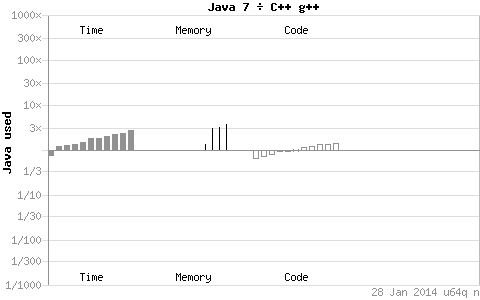
\includegraphics[width=.7\textwidth]{images/java-cpp-performance.png}

{\tiny\url{http://benchmarksgame.alioth.debian.org/u64q/benchmark.php?test=all&lang=java&id=5&data=u64q}}
\end{center}
\end{frame}

\section{Uso industrial}

\begin{frame}[t]{Popularidad}
\begin{center}
\begin{tabular}{|l|r|}
\hline
\textbf{Lenguaje} & \textbf{Cuota de popularidad}\\
\hline
C & 17.871\%\\
\hline
Java & 16.499\%\\	
\hline
Objective-C & 11.098\%\\
\hline
C++ & 7.548\%\\
\hline
C\# & 5.855\%\\	
\hline
PHP & 4.627\%\\
\hline
(Visual) Basic & 2.989\%\\
\hline
Python & 2.400\%\\
\hline
JavaScript & 1.569\%\\
\hline
Transact-SQL & 1.559\%\\
\hline
\end{tabular}
\vfill
{\tiny Fuente: TIOBE Index, enero de 2013}
\end{center}
\end{frame}

\begin{frame}[t]{Sistemas Operativos}
  \begin{itemize}
    \item Microsoft Windows: C, C++.
    \item Linux: C.
    \item Apple MacOS: C, C++, Objective-C.
    \item Sun Solaris: C.
    \item HP-UX: C.
    \item Apple iOS: C, C++, Objective-C.
    \item Google Android: C, Java.
    \item RIM Blackberry OS 4.x: C++.
    \item Amazon Kindle	OS: C.
  \end{itemize}
  \vfill
  {\tiny Fuente: http://www.lextrait.com/vincent/implementations.html}
\end{frame}

\begin{frame}[t]{Interfaz gráfica}
  \begin{itemize}
    \item Microsoft Windows UI: C++.
    \item Apple MacOS (Aqua): C++.
    \item Gnome: C.
    \item KDE: C++.
  \end{itemize}
  \vfill
  {\tiny Fuente: http://www.lextrait.com/vincent/implementations.html}
\end{frame}

\begin{frame}[t]{Ofimática}
  \begin{itemize}
    \item Microsoft Office: C++.
    \item Apache Open Office: C++.
    \item Corel Office: C++.
    \item Adobe Acrobat: C++.
    \item Evernote: C++.
  \end{itemize}
  \vfill
  {\tiny Fuente: http://www.lextrait.com/vincent/implementations.html}
\end{frame}

\begin{frame}[t]{Clientes de Internet}
  \begin{itemize}
    \item Navegadores Web:
      \begin{itemize}
        \item Microsoft Internet Explorer: C++.
        \item Mozilla Firefox: C++.
        \item Safari: C++.
        \item Google Chrome: C++.
        \item Opera: C++.
        \item Opera Mini: C++, Java, Pike.
        \item Mosaic: C.
      \end{itemize}
    \item Correo electrónico:
      \begin{itemize}
        \item Microsoft Outlook: C++.
        \item IBM Lotus Notes: C.
      \end{itemize}
    \end{itemize}
  \vfill
  {\tiny Fuente: http://www.lextrait.com/vincent/implementations.html}
\end{frame}

\begin{frame}[t]{Software de servidor}
  \begin{itemize}
    \item Bases de datos:
      \begin{itemize}
        \item Oracle: C++.
        \item MySQL: C++.
        \item IBM DB2: C.
        \item Microsoft SQL Server: C++.
        \item IBM Informix: C.
        \item SAP DB: C++.
      \end{itemize}
    \item Servidores Web:
      \begin{itemize}
        \item Apache: C, C++.
        \item Microsoft IIS: C++.
      \end{itemize}
  \end{itemize}
  \vfill
  {\tiny Fuente: http://www.lextrait.com/vincent/implementations.html}
\end{frame}

\begin{frame}[t]{Sitios Web}
  \begin{itemize}
    \item eBay: Java.
    \item PayPal: C++.
    \item Amazon: C++, Java.
    \item facebook: C++, PHP.
    \item Youtube: Python.
    \item Dropbox: Python.
  \end{itemize}
  \vfill
  {\tiny Fuente: http://www.lextrait.com/vincent/implementations.html}
\end{frame}

\begin{frame}[t]{Nichos de utilización}
  \begin{itemize}
    \item ¿Hay un lugar para lenguajes basados en máquina virtual?
      \begin{itemize}
        \item Aplicaciones ejecutadas en un servidor de aplicaciones.
        \item Aplicaciones sin requisitos estrictos de rendimiento.
        \item Aplicaciones sin restricciones de consumo de memoria.
      \end{itemize}
    \item ¿Tienen sentido los lenguajes basados en máquina virtual para aplicaciones de escritorio?
      \begin{itemize}
        \item La mayoría de los intentos han fracasado.
      \end{itemize}
    \item ¿Y para aplicaciones en dispositivos móviles?
      \begin{itemize}
        \item Google Android es un ejemplo.
        \item Pero si hace falta rendimiento o hay problemas de memoria se acaba recurriendo al NDK.
      \end{itemize}
  \end{itemize}
\end{frame}

\section{Uso docente}

\begin{frame}[t]{Las JavaSchools}
  \begin{itemize}
    \item Una escuela Java se caracteriza por:
      \begin{itemize}
        \item Utiliza Java como primer lenguaje de programación.
        \item Ilustra en la mayoría de las asignaturas los conceptos mediante Java.
        \item Presta poca atención a paradigmas distintos de la orientación a objetos.
      \end{itemize}
    \pause
    \item Problema:
      \begin{itemize}
        \item La evolución de las tecnologías informáticas es demasiado rápida para hacer formación a corto plazo.
        \item La preparación universitaria debe centrarse en el medio y largo plazo.
      \end{itemize}
  \end{itemize}
\end{frame}

\begin{frame}[t]{Primer lenguaje}
  \begin{itemize}
    \item La gestión automática de memoria simplifica la programación.
      \begin{itemize}
        \item Pero los estudiante nos adquieren el patrón mental de adquisición/liberación.
        \item Es un patrón que va mucho más allá de la gestión de memoria.
      \end{itemize}
    \item \pause El modelo basado en máquina virtual oculta muchos detalles de la ejecución del programa.
      \begin{itemize}
        \item Esto favorece la confusión de conceptos que deben separarse claramente.
        \item Traducción, código fuente, código objeto, código ejecutable, compilación, enlace, ...
      \end{itemize}
    \item \pause El estudiante no adquiere preocupación por el rendimiento y la gestión responsable de recursos.
  \end{itemize}
\end{frame}

\begin{frame}[t]{(casi) Único lenguaje}
  \begin{itemize}
    \item A favor:
      \begin{itemize}
        \item Las asignaturas pueden centrarse en sus contenidos propios porque el alumno ya conoce el lenguaje.
        \item El estudiante acaba siendo un experto en el lenguaje.
      \end{itemize}
    \item \pause En contra:
      \begin{itemize}
        \item El estudiante no adquiere competencias para enfrentarse a situaciones nuevas o desconocidas.
        \item El estudiante intenta resolver todo tipo de problemas con una única herramienta.
        \item ¿ Y si no encuentra una solución razonable con el lenguaje?
        \item Factor limitante en el tipo de puestos a los que el titulado puedo optar.
      \end{itemize}
  \end{itemize}
\end{frame}

\begin{frame}[t]{Único paradigma}
  \begin{itemize}
    \item La Programación Orientada a Objetos es un paradigma de programación originado a finales de los 60.
      \begin{itemize}
        \item No es el único paradigma de programación.
        \item No se adapta bien a todos los problemas.
      \end{itemize}
  \end{itemize}
\end{frame}


\section{¿Y ahora qué?}

\begin{frame}
\titlepage
\end{frame}

\end{document}
